% Chapter 1

\chapter{Overview} % Main chapter title

\label{Chapter1} % For referencing the chapter elsewhere, use \ref{Chapter1} 

\lhead{Chapter 1. \emph{Overview}} % This is for the header on each page - perhaps a shortened title

%----------------------------------------------------------------------------------------
\section{Introduction}
For decades, the keyboard and mouse have been the standard interface mechanisms of input for computer systems. Their legacy is apparent in the applications that have been designed with the purpose of maximizing their efficiency and effectiveness. However, as technology advances, new mechanisms have been created in the hopes of making interactions with computer systems less rigid. While the keyboard and mouse interface are less physically demanding on the body in order to carry out commands, they do not allow for an expressive range of motion. The keyboard and mouse are only expressive in two dimensions as they are limited to up, down or right, left movements of the mouse across a computer screen. The keyboard is even less expressive than the mouse as the user must use key strokes to carry out commands, thus making the mouse slightly more fluid in motion than the keyboard but not by much. The interfaces have stayed relatively the same despite advances in computer software and hardware. With the advent of tablets and smart devices, the envelope had been pushed in terms of what could be considered "effective" means of input for a computer system. These devices allow for a user to carry out a command with a simple stroke of their finger directly on the screen of their computer system, thus making the command more expressive than the traditional keyboard and mouse interface. The devices with touchscreen capabilities have opened the door for opportunities to create a fresh interface.A new interface may have the ability to replace the use of a keyboard and mouse or augment the way we interact with digital information while offering an even greater, more expressive range of motion to the user in a more "hands-off" capacity. The term "hands-off" referring to the fact that the keyboard and mouse interface as well as the touchscreen interface both require the user to literally be touching a device of some sort in order to carry out a command. However, certain interface technologies were created with the intention of never having to place one's hands on a device.

With these ideas in mind, the project set out with the simple goal of developing an application for children by children using an interface with these specifications. The interface chosen was LeapMotion.


\begin{figure}
\centering
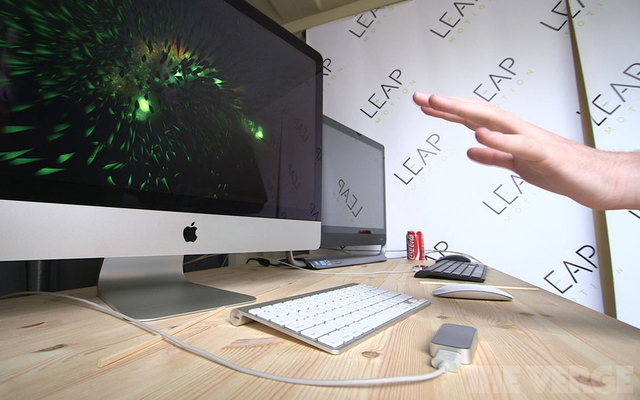
\includegraphics[ height=0.5\textwidth, width=0.65\textwidth]{leap-exp-watermark-rm-vrg_large_verge_medium_landscape}
\caption{Interacting with the LeapMotion. \cite{theverge} }
\label{fig:leapmotionpicture}
\end{figure}

\section{LeapMotion}

The LeapMotion is a small device that can fit in the palm of your hand which sits in front of a monitor as seen in Figure~\ref{fig:leapmotionpicture} and captures motion in 3 cubic feet of space using a pair of cameras. The small cameras triangulate the positions of hands, fingers and tools in their relative space between the LeapMotion and the monitor relaying accurate position and velocity data in real time. The data can then be used to control application by driving the user interface of the system. \cite{leapmotion} 

This type of interaction with the computer system is different from the traditional keyboard and mouse because it does not require any physical contact with objects connected to the system and has the ability to sense a much wider range of input. The LeapMotion is also expressive in three dimensions as opposed to two.

\begin{figure}
\centering
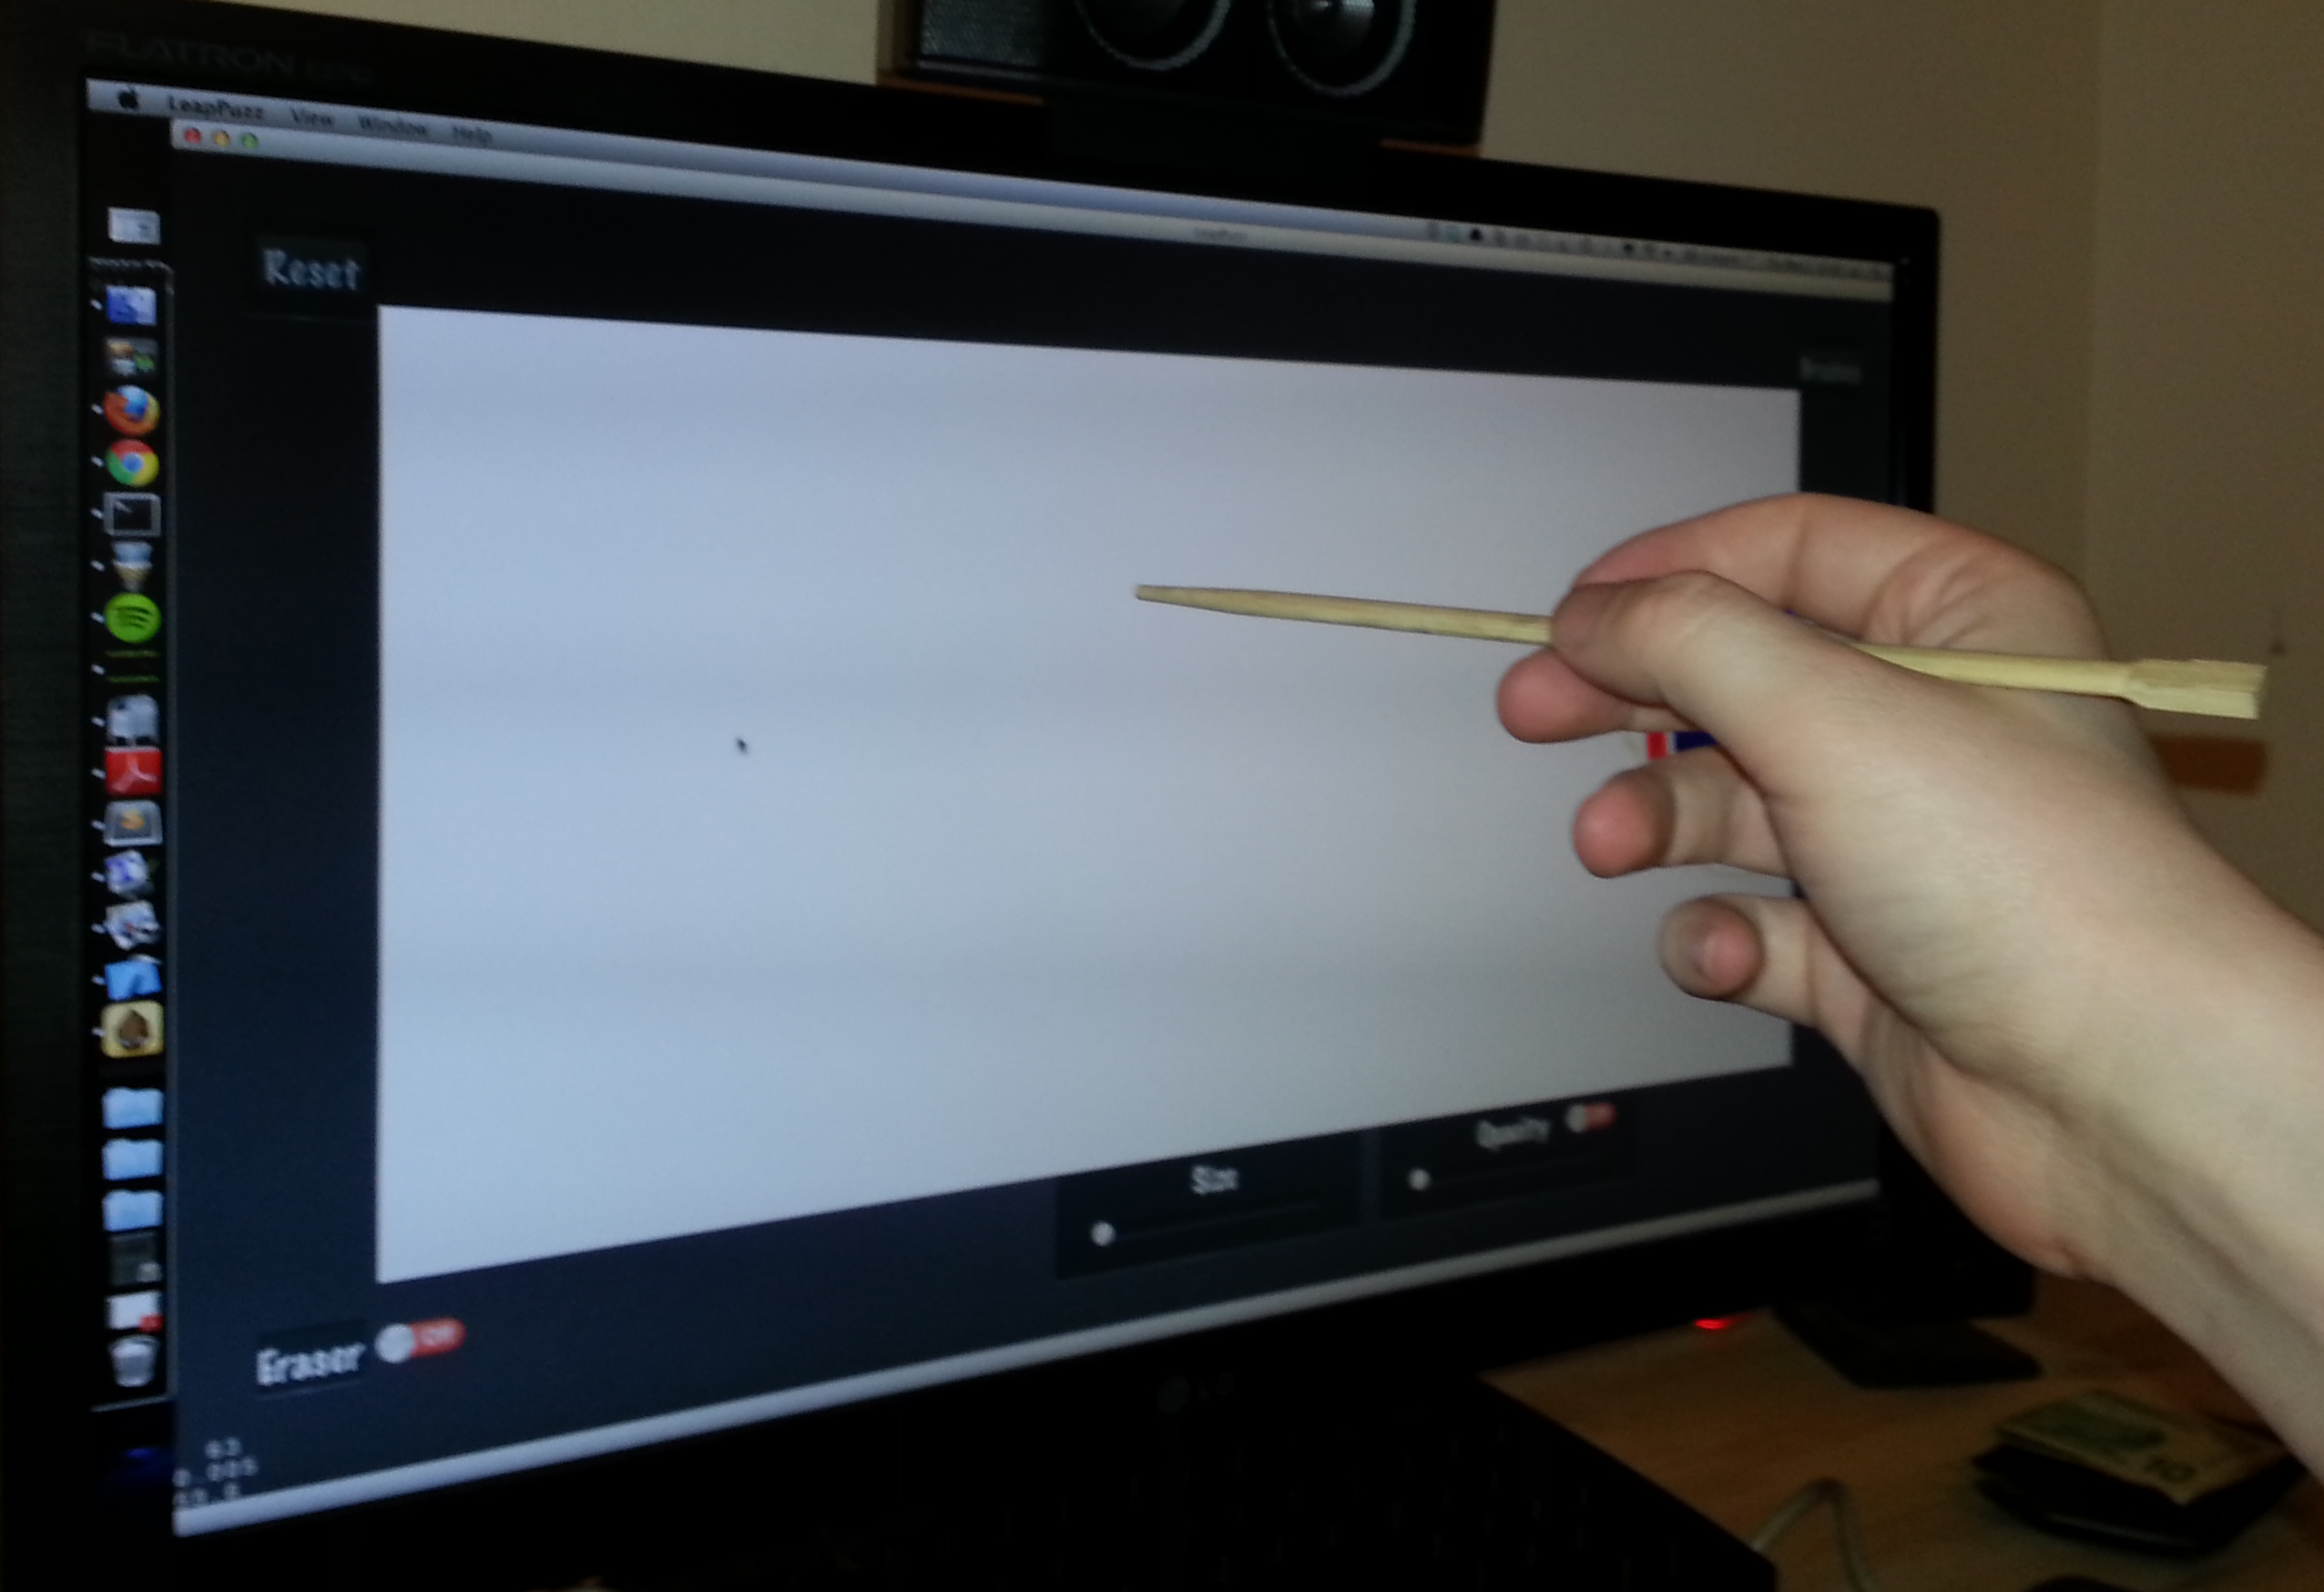
\includegraphics[ height=0.5\textwidth, width=0.75\textwidth]{chopstick}
\caption{Using a chopstick as a pointer}
\label{fig:chopstick}
\end{figure}
In this paper and throughout the project we refer to a finger or tool interacting with LeapMotion as a "pointer\footnote{The documentation refers to this as a "pointable"}." The tool can be any object is "stick-like" such as a pen, pencil or chopstick. Throughout this project a chopstick was mostly used as seen in Figure~\ref{fig:chopstick} as the preferable tool. Initially it was intended for the application to track fingers although through development and testing it was found that tracking fingers was not as reliable as rigid tool. Tracking was less reliable for the childrens smaller sporadically moved hands.

\section{Project Scope}
Although we wanted to see if the keyboard and mouse could be replaced by the LeapMotion there are some functions that we understand would almost be certainly not possible. Tasks that require the user to type large amounts of information, such as data entry or word processing, are two such examples of exceptions we will not be focusing on in this project. The focus, therefore, would be on some of the other functions the keyboard may serve such as switching applications which can be performed by the keyboard shortcut ALT + TAB or with a mouse. The LeapMotion might be able to replace this functionality with a wave of a hand indicating to switch the applications automatically in carousel. 
